\newpage
\subsection{Importing and working with multiple EAPs}
\visHeader
\label{sec:multiEAP}

Before starting, it should be mentioned that the following instructions are how to properly export and import Enterprise Architect (EA) files. This is not an
eMoflon exclusive feature. You may want to bookmark this section so that you can reference it later as it's important to be able to import a different EAP into
the same project.

\begin{itemize}

\item[$\blacktriangleright$] In the same \texttt{Part4.zip} folder you extracted this document from, double-click on \texttt{DictionaryLanguageSource.eap} to
open the file in EA.

\item[$\blacktriangleright$] The expanded rootnote should resemble Fig.~\ref{fig:dictionaryLangStart}. While you are able to copy and paste packages between
multiple EAPs (i.e., copy \texttt{<<EPack\-age>>DictionaryLanguage} into the \texttt{MyWorkingSet} root note of \texttt{Leit\-nersLearningBox}), if any of the
copied packages have dependencies on other packages, it cannot be done so easily. All links would be destroyed! If you tried to copy the dictionary language,
for example, the receiving project would not be able to establish the neccesary links to eMoflon's \texttt{Moca Language}.

\begin{figure}[htbp]
\begin{center}
  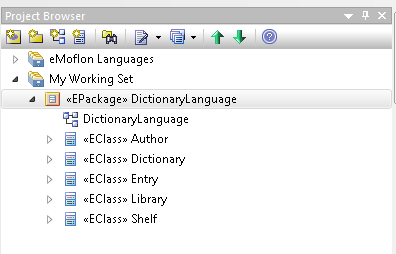
\includegraphics[width=0.4\textwidth]{ea_dictLangProBrowser}
  \caption{caption}
  \label{fig:dictionaryLangStart}
\end{center}
\end{figure}

\item[$\blacktriangleright$] Therefore, to migrate multiple packages, you have to first export a \emph{complete} root node to an XMI file. First right-click on
the EPackage \texttt{DictionaryLanguage}, then navigate to ``Import/Export / Export Model to XMI\ldots'' (Fig.~\ref{fig:contextExport}). Alternatively, select
the root and press \texttt{Ctrl + Alt + E}.

\begin{figure}[htbp]
\begin{center}
  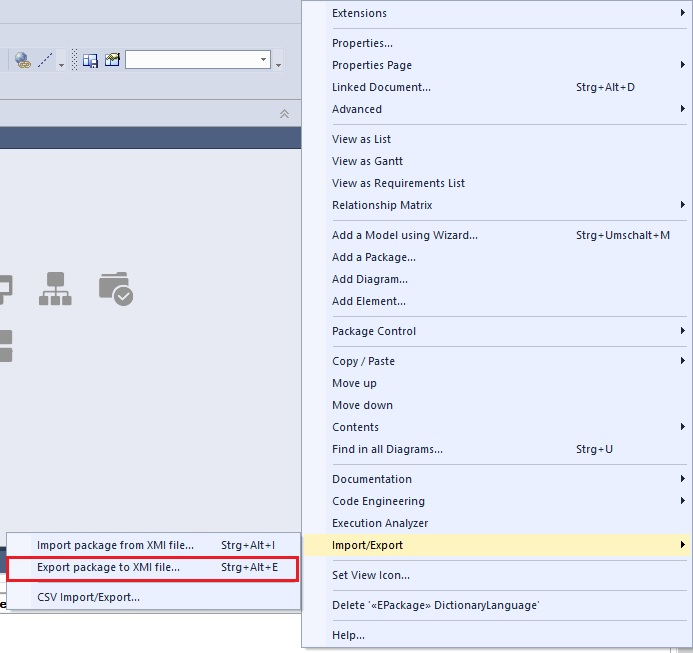
\includegraphics[width=\textwidth]{ea_contextExport}
  \caption{caption}
  \label{fig:contextExport}
\end{center}
\end{figure}

\item[$\blacktriangleright$] Save the file somewhere easily accessible, such as your desktop, and change the export type to \texttt{XMI 2.1}. Press export,
and close the window once the small green bar appears (Fig.~\ref{fig:export}).

\vspace{0.5cm}

\begin{figure}[htbp]
\begin{center}
  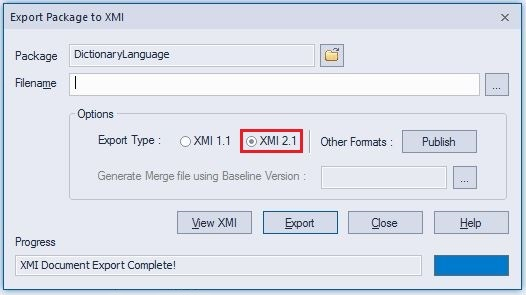
\includegraphics[width=0.9\textwidth]{ea_dialogueExport}
  \caption{caption}
  \label{fig:export}
\end{center}
\end{figure}

\item[$\blacktriangleright$] Now open \texttt{LeitnersLearningBox.eap} from Eclipse and right-click anywhere in the project browser. Navigate to ``Import
Model from XMI\ldots''

\item[$\blacktriangleright$] Find the \texttt{.xmi} file you just saved and press \texttt{import}. Press \texttt{OK} in the confirmation dialogue. Your project
browser now resemble Fig.~\ref{fig:importProBrowser}.

\begin{figure}[htbp]
\begin{center}
  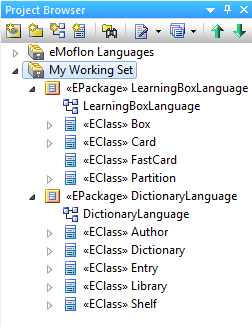
\includegraphics[width=0.4\textwidth]{ea_importedProjectBrowser}
  \caption{caption}
  \label{fig:importProBrowser}
\end{center}
\end{figure}

\item[$\blacktriangleright$] The final step is to validate and export both metamodels to Eclipse! First, use the eMolfon control panel to and under
\texttt{Validate}, press \texttt{All}.\footnote{To review the details and how to use the eMoflon control panel, read Section 2.8 from Part II}

\item[$\blacktriangleright$] Switch back to Eclipse and refresh your package explorer. A new \texttt{DictionaryLanguage} project should have appeared under
\texttt{My Working Set}.

\item[$\blacktriangleright$] Thats everything! You're now ready to start using your source and target metamodels with TGGs. If you've just joined us and are
interested in the eMoflon project structure, or curious as to how Java code is generated from your visual metamodel, we invite you to read Part I, Section 4.1.
Otherwise, continue with this part to start developing your TGG Schema.

\jumpSingle{TGGSchema}

\end{itemize}
